\section{Elementary Data Structures}
\subsection{Stacks and queues}
\label{sub:stacks_and_queues}



\begin{description}

\descitem{10.1-1} \textit{Using Figure 10.1 as a model, illustrate the result of each operation in the sequence $\proc{Push}(S,4)$, $\proc{Push}(S,1)$,$\proc{Push}(S,3)$, $\proc{Pop}(S)$, $\proc{Push}(S,8)$, and $\proc{Pop}(S)$  on an initially empty stack $S$ stored in array $S[1 \twodots6]$.}
\begin{ex}
    \begin{figure}[H]
      \centering
      \begin{subfigure}[t]{.45\textwidth}
        \centering
        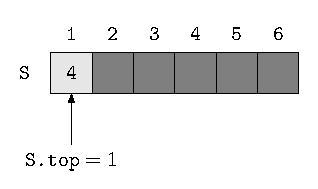
\includegraphics[scale=1]{img/10_1-1/10_1-1_1.pdf}
        \caption{$\proc{Push}(S,4)$}\label{fig:10_1-1_1}
      \end{subfigure}
      \begin{subfigure}[t]{.45\textwidth}
        \centering
        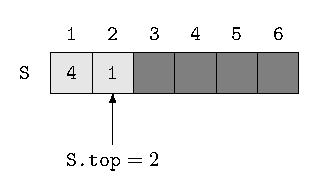
\includegraphics[scale=1]{img/10_1-1/10_1-1_2.pdf}
        \caption{$\proc{Push}(S,1)$}\label{fig:10_1-1_2}
      \end{subfigure}
      \begin{subfigure}[t]{.45\textwidth}
        \centering
        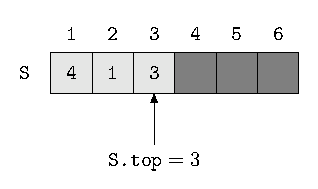
\includegraphics[scale=1]{img/10_1-1/10_1-1_3.pdf}
        \caption{$\proc{Push}(S,3)$}\label{fig:10_1-1_3}
      \end{subfigure}
      \begin{subfigure}[t]{.45\textwidth}
        \centering
        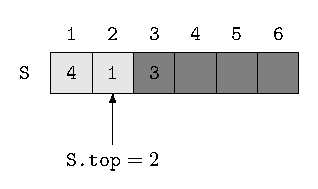
\includegraphics[scale=1]{img/10_1-1/10_1-1_4.pdf}
        \caption{$\proc{Pop}(S)$}\label{fig:10_1-1_4}
      \end{subfigure}
      \begin{subfigure}[t]{.45\textwidth}
        \centering
        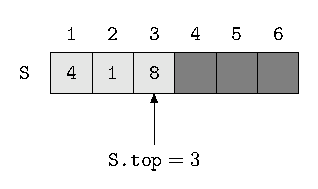
\includegraphics[scale=1]{img/10_1-1/10_1-1_5.pdf}
        \caption{$\proc{Push}(S,8)$}\label{fig:10_1-1_5}
      \end{subfigure}
      \begin{subfigure}[t]{.45\textwidth}
        \centering
        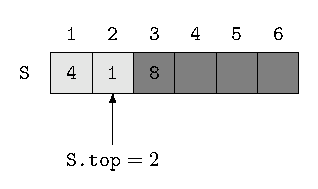
\includegraphics[scale=1]{img/10_1-1/10_1-1_6.pdf}
        \caption{$\proc{Pop}(S)$}\label{fig:10_1-1_6}
      \end{subfigure}
      \caption{Séquence d'opérations sur une pile vide de taille 6.} 
      \label{fig:stack-seq} 
    \end{figure}
\end{ex}
\descitem{10.1-2} \textit{Explain how to implement two stacks in one array $A[1\twodots n]$ in such a way that neither stack overflows unless the total number of elements in both stacks together is $n$. The \proc{Push} and \proc{Pop} operations should run in $O(1)$ time.}
\begin{ex}
  Il suffit d'initialiser les piles aux extrémités du tableau, \textit{i.e.} $S_1.\textrm{top} = 1$ et $S_2.\textrm{top} = n$. La pile $S_1$ fonctionne comme montré à la fig. \ref{fig:stack-seq} et la pile $S_2$ décrémente l'indice du sommet lors d'un \proc{Push} et l'incrémente lors d'un \proc{Pop}. Lorsque le nombre total des éléments des deux piles est égale à $n$, il y a overflow si on empile un élément dans une des piles. Les primitives \proc{Push} et \proc{Pop} sont bien de $O(1)$.
  %TODO:Tikz:illustration ?
\end{ex}
\descitem{10.1-3} \textit{Using Figure 10.2 as a model,  illustrate the result of each operation in the sequence $\proc{Enqueue}(Q, 4)$, $\proc{Enqueue}(Q, 1)$, $\proc{Enqueue}(Q, 3)$, $\proc{Dequeue}(Q)$,  $\proc{Enqueue}(Q, 8)$,  and $\proc{Dequeue}(Q)$ on an initially empty queue $Q$ stored in array $Q[1 \twodots 6]$.}
\begin{ex}
  
    \begin{figure}[H]
      \centering
      \begin{subfigure}[t]{.45\textwidth}
        \centering
        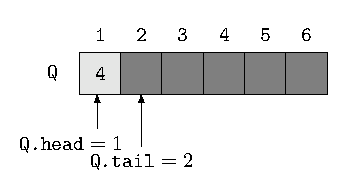
\includegraphics[scale=1]{img/10_1-3/10_1-3_1.pdf}
        \caption{$\proc{Enqueue}(Q,4)$}\label{fig:10_1-3_1}
      \end{subfigure}
      \begin{subfigure}[t]{.45\textwidth}
        \centering
        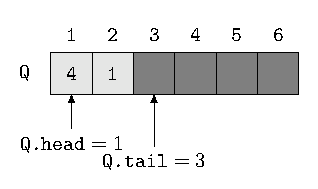
\includegraphics[scale=1]{img/10_1-3/10_1-3_2.pdf}
        \caption{$\proc{Enqueue}(Q,1)$}\label{fig:10_1-3_2}
      \end{subfigure}
      \begin{subfigure}[t]{.45\textwidth}
        \centering
        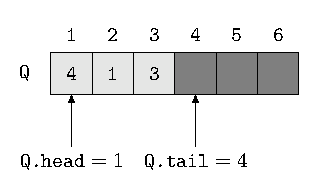
\includegraphics[scale=1]{img/10_1-3/10_1-3_3.pdf}
        \caption{$\proc{Enqueue}(Q,3)$}\label{fig:10_1-3_3}
      \end{subfigure}
      \begin{subfigure}[t]{.45\textwidth}
        \centering
        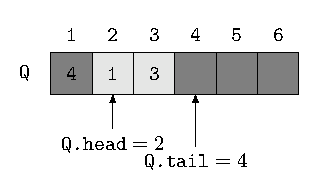
\includegraphics[scale=1]{img/10_1-3/10_1-3_4.pdf}
        \caption{$\proc{Dequeue}(Q)$}\label{fig:10_1-3_4}
      \end{subfigure}
      \begin{subfigure}[t]{.45\textwidth}
        \centering
        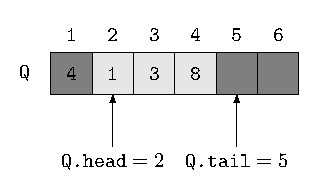
\includegraphics[scale=1]{img/10_1-3/10_1-3_5.pdf}
        \caption{$\proc{Enqueue}(Q,8)$}\label{fig:10_1-3_5}
      \end{subfigure}
      \begin{subfigure}[t]{.45\textwidth}
        \centering
        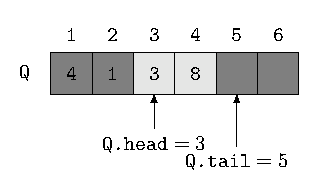
\includegraphics[scale=1]{img/10_1-3/10_1-3_6.pdf}
        \caption{$\proc{Dequeue}(Q)$}\label{fig:10_1-3_6}
      \end{subfigure}
      \caption{Séquence d'opérations sur une file vide de taille 6.} 
      \label{fig:queue-seq} 
    \end{figure}
\end{ex}
\descitem{10.1-4} \textit{Rewrite \proc{Enqueue} and \proc{Dequeue} to detect underflow and overflow of a queue.}
\begin{ex}
  La description donnée ne permet pas de déterminer si une file est vide ou pleine. Supposons, par commodité, que la file est implémenté sur le tableau $Q[0\twodots n-1]$ (cette hypothèse est pratique pour l'arithmétique modulaire). Il existe plusieurs méthodes possibles pour contourner ce problème, on en présente ici trois :
  \begin{enumerate}[label=\circled{\arabic*}]
    \item Ajouter en attribue de la file un état \textit{isempty} qui vaut \const{true} si la file est vide et \const{false} inversement. La file est pleine lorsque $\attrib{Q}{head} = \attrib{Q}{tail}$ et $\attrib{Q}{isempty} = \const{false}$.

\begin{codebox}
\Procname{\textbf{Algorithme}\quad\textsc{Enqueue-1}$(\id{Q}, \id{e})$}
    \li \If $\attrib{Q}{head}\isequal\attrib{Q}{tail} \And \attrib{Q}{isempty} \isequal \const{false}$ \Then
        \li \Error "The queue is full : failed to enqueue." \End
    \li  $Q[\attrib{Q}{tail}] \gets e$ 
    \li $\attrib{Q}{tail} = (\attrib{Q}{tail}+1)\bmod \attrib{Q}{length}$
    \li \If $\attrib{Q}{isempty} \isequal \const{true}$ \Then
      \li $\attrib{Q}{isempty} \gets \const{false}$ \End
\end{codebox}
\begin{codebox}
\Procname{\textbf{Algorithme}\quad\textsc{Dequeue-1}$(\id{Q})$}
    \li \If $\attrib{Q}{isempty}$ \Then
        \li \Error "The queue is empty: failed to dequeue." \End
    \li  $\id{e} \gets Q[\attrib{Q}{head}]$ 
    \li $\attrib{Q}{head} = (\attrib{Q}{head}+1)\bmod \attrib{Q}{length}$
    \li \If $\attrib{Q}{head} \isequal \attrib{Q}{tail}$ \Then
      \li $\attrib{Q}{isempty} \gets \const{true}$ \End
    \li \Return \id{e}
\end{codebox}
    \item Faire pointer $\attrib{Q}{head}$ vers \const{Nil} si la file est vide. La file est pleine lorsque $\attrib{Q}{head} = \attrib{Q}{tail}$.
\begin{codebox}
\Procname{\textbf{Algorithme}\quad\textsc{Enqueue-2}$(\id{Q}, \id{e})$}
    \li \If $\attrib{Q}{head}\isequal\attrib{Q}{tail}$ \Then
        \li \Error "The queue is full : failed to enqueue." \End
    \li  $Q[\attrib{Q}{tail}] \gets e$ 
    \li $\attrib{Q}{tail} = (\attrib{Q}{tail}+1)\bmod \attrib{Q}{length}$
\end{codebox}
\begin{codebox}
\Procname{\textbf{Algorithme}\quad\textsc{Dequeue-2}$(\id{Q})$}
    \li \If $\attrib{Q}{head}\isequal\const{Nil}$ \Then
        \li \Error "The queue is empty: failed to dequeue." \End
    \li  $\id{e} \gets Q[\attrib{Q}{head}]$ 
    \li $\attrib{Q}{head} = (\attrib{Q}{head}+1)\bmod \attrib{Q}{length}$
    \li \If $\attrib{Q}{head} \isequal \attrib{Q}{tail}$ \Then
      \li $\attrib{Q}{head} \gets \const{Nil}$ \End
    \li \Return \id{e}
\end{codebox}
    \item \footnote{L'implémentation des algorithmes suivantes se trouve dans le dossier \pathx{code/CH10_Elementary_Data_Structures/Queue/}.}
    À la place de $\attrib{Q}{head}$ et $\attrib{Q}{tail}$, on utilise $\attrib{Q}{front}$ et $\attrib{Q}{count}$. $\attrib{Q}{front}$ joue le même rôle que $\attrib{Q}{tail}$. L'emplacement de $\attrib{Q}{head}$ peut se déduire à partir de l'identité :
        \[\attrib{Q}{head} + \attrib{Q}{count}\equiv \attrib{Q}{tail}\pmod{\attrib{Q}{length}}.\]
    Dans ce cas, la file est vide si $\attrib{Q}{count} = 0$ et pleine si $\attrib{Q}{count} = \attrib{Q}{length}$. 
\begin{codebox}
\Procname{\algo{Enqueue-With-Counter}$(\id{Q}, \id{e})$}
    \li \If $\attrib{Q}{count}\isequal\attrib{Q}{length}$ \Then
        \li \Error "The queue is full : failed to enqueue." \End
    \li  $Q[\attrib{Q}{front}] \gets e$ 
    \li $\attrib{Q}{count} = \attrib{Q}{count}+1$
    \li $\attrib{Q}{front} = (\attrib{Q}{front}+1)\bmod \attrib{Q}{length}$
\end{codebox}
\begin{codebox}
\Procname{\algo{Dequeue-With-Counter}$(\id{Q})$}
    \li \If $\attrib{Q}{count}\isequal0$ \Then
        \li \Error "The queue is empty: failed to dequeue." \End
    \li  $\id{e} \gets Q[(\attrib{Q}{front} - \attrib{Q}{count} + \attrib{Q}{length}) \bmod \attrib{Q}{length}]$ \label{li:dequeue-counter-tail}
    \li  $\attrib{Q}{count} = \attrib{Q}{count}-1$
    \li \Return \id{e}
\end{codebox}
\textit{N.B.} À la ligne \ref{li:dequeue-counter-tail} de l'algorithme \textsc{Dequeue-With-Counter}, on ajoute $\attrib{Q}{length}$ pour assurer que l'indice soit positive. 
  \end{enumerate} 
\end{ex}
\descitem{10.1-5} \textit{Whereas a stack allows insertion and deletion of elements at only one end, and a queue allows insertion at one end and deletion at the other end, a \textbf{deque} (double-ended queue) allows insertion and deletion at both ends. Write four $O(1)$-time procedures to insert elements into and delete elements from both ends of a deque implemented by an array.}
\begin{ex}
   On reprend les algorithmes \textsc{Enqueue-With-Counter} et \textsc{Dequeue-With-Counter} et les attribues définies. Les algorithmes suivantes complètent une file à une \textit{deque}.\footnote{L'implémentation des algorithmes suivantes se trouve dans le dossier \pathx{code/CH10_Elementary_Data_Structures/Deque/}.}
\begin{codebox}
\Procname{\algo{Enqueue-At-Other-End}$(\id{Q}, \id{e})$}
    \li \If $\attrib{Q}{count}\isequal\attrib{Q}{length}$ \Then
        \li \Error "The queue is full : failed to enqueue." \End
    \li  $Q[(\attrib{Q}{front} - (\attrib{Q}{count} + 1) + \attrib{Q}{length}) \bmod \attrib{Q}{length}] \gets e$ 
    \li $\attrib{Q}{count} = \attrib{Q}{count}+1$
\end{codebox}
\begin{codebox}
\Procname{\algo{Dequeue-At-Other-End}$(\id{Q})$}
    \li \If $\attrib{Q}{count}\isequal0$ \Then
        \li \Error "The queue is empty: failed to dequeue." \End
    \li  $\attrib{Q}{front} \gets (\attrib{Q}{front} -1 + \attrib{Q}{length}) \bmod \attrib{Q}{length}$
    \li  $\id{e} \gets Q[\attrib{Q}{front}]$ 
    \li  $\attrib{Q}{count} = \attrib{Q}{count}-1$
    \li \Return \id{e}
\end{codebox}
\end{ex}
\descitem{10.1-6} \textit{Show how to implement a queue using two stacks. Analyse the running time of the queue operations.}
\descitem{10.1-7} \textit{Show how to implement a stack using two queues. Analyse the running time of the queue operations.}


\end{description}

\subsection{Linked lists}
\label{sub:linked_lists}


